
\section{Auswertung von Messvergleichen mit Referenzlabor}
In dieser Vorlesung wird die Anwendung des t-Tests und des Chi2-Tests auf eines der zentralen Themen der Metrologie gezeigt, 
welches die Durchführung von Ringvergleichen ist. Wesen der Metrologie ist, dass Messgrößen auf die SI-Einheiten zurückgeführt werden, 
damit sie weltweit vergleichbar sind. Um die Vergleichbarkeit von Ergebnissen unterschiedlicher gesetzlich geprüfter Laboratorien, seien dies Staatsinstitute verschiedener Länder oder Kalibrierlaboratorien innerhalb eines Landes, zu gewährleisten, werden Ringvergleiche durchgeführt.
Dazu wird beispielsweise ein Messobjekt (Prüfkörper) rumgeschickt und jedes beteiligte Labor misst an demselben Objekt eine genau spezifizierte Messgröße nach einem vorgegebenen Verfahren. Um die Ergebnisse miteinander zu vergleichen, werden die statistischen Verfahren der Hypothesentests auf Gleichheit der Mittelwerte und der Standard\-ab\-weichungen eingesetzt.

Es wird bei der Verwendung des t-Tests danach unterschieden, ob die Nullhypothese getestet wird, dass Mittelwerte der Laboratorien mit einem Erwartungswert (dem Referenzwert) übereinstimmen.
Der Referenzwert wird beispielsweise von einem Referenzlabor zur Verfügung gestellt, das die Möglichkeit hatte, mit deutlich mehr Aufwand und genaueren Geräten, messen zu können.
Für den Vergleich wird die zu vergleichende Messgröße normiert, wie wir es in der letzten Vorlesung schon kennengelernt hatten.

Wir betrachten die Messergebnisse mit Größenwerten $x_i$ für $i = 1,\dots,N$ und Unsicherheiten $u_i$ von $N$ Laboratorien (Partner des Ringvergleichs).

Die standardnormalverteilen Zufallsgrößen, die die Differenz zwischen dem Ergebnis eines Labors bezogen auf den Referenzwert repräsentieren, werden auch Z-Scores oder Z-Werte genannt. Sie werden genutzt, wenn z.~B. das Messergebnis eines
Partners $i$ mit dem Referenzwert (Erwartungswert) verglichen werden soll.
Liegt das Messergebnis des Partners $i$ oberhalb des Referenzwertes, so ist der Z-Wert positiv.
Liegt das Messergebnis  unterhalb des Erwartungswertes, so ist der Z-Wert negativ. 
Um den Z-Wert zu bestimmen, müssen der Erwartungswert $\mu$ und die 
Standardabweichung $\sigma$ der zu Grunde liegenden Verteilung 
bekannt sein. Es reicht nicht aus nur die empirischen Werte (empirischer Erwartungswert, d.h.\
Mittelwert, und empirische Standardabweichung) aus den Stichproben zu schätzen.
Ist $X$ eine Zufallsvariable mit dem Erwartungswert $\mathrm{E}(X)=\mu$ und 
der Varianz $\mathrm{Var}(X) = \sigma^2$ erhält man die zugehörige normierte Zufallsgröße $Z$ durch:
\begin{equation}
Z=\frac{X-\mu}{\sigma}
\end{equation}
Für den Erwartungswert und die Varianz von $Z$ gilt:
\begin{itemize}
	\item $\mathrm{E}(Z) = \mathrm{E}\left( \frac{X-\mu}{\sigma} \right) =
	\frac{1}{\sigma} (\mathrm{E}(X) -\mu) = 0$
	\item $\mathrm{Var}(Z) = \mathrm{Var} \left(\frac{X-\mu}{\sigma} \right) = 
	\mathrm{Var} \left(\frac{X-\mu}{\sigma} \right) = 
	\frac{1}{\sigma^2} \mathrm{Var}(X) = 1$
\end{itemize}

\begin{figure}[!htp]
	\begin{center}
		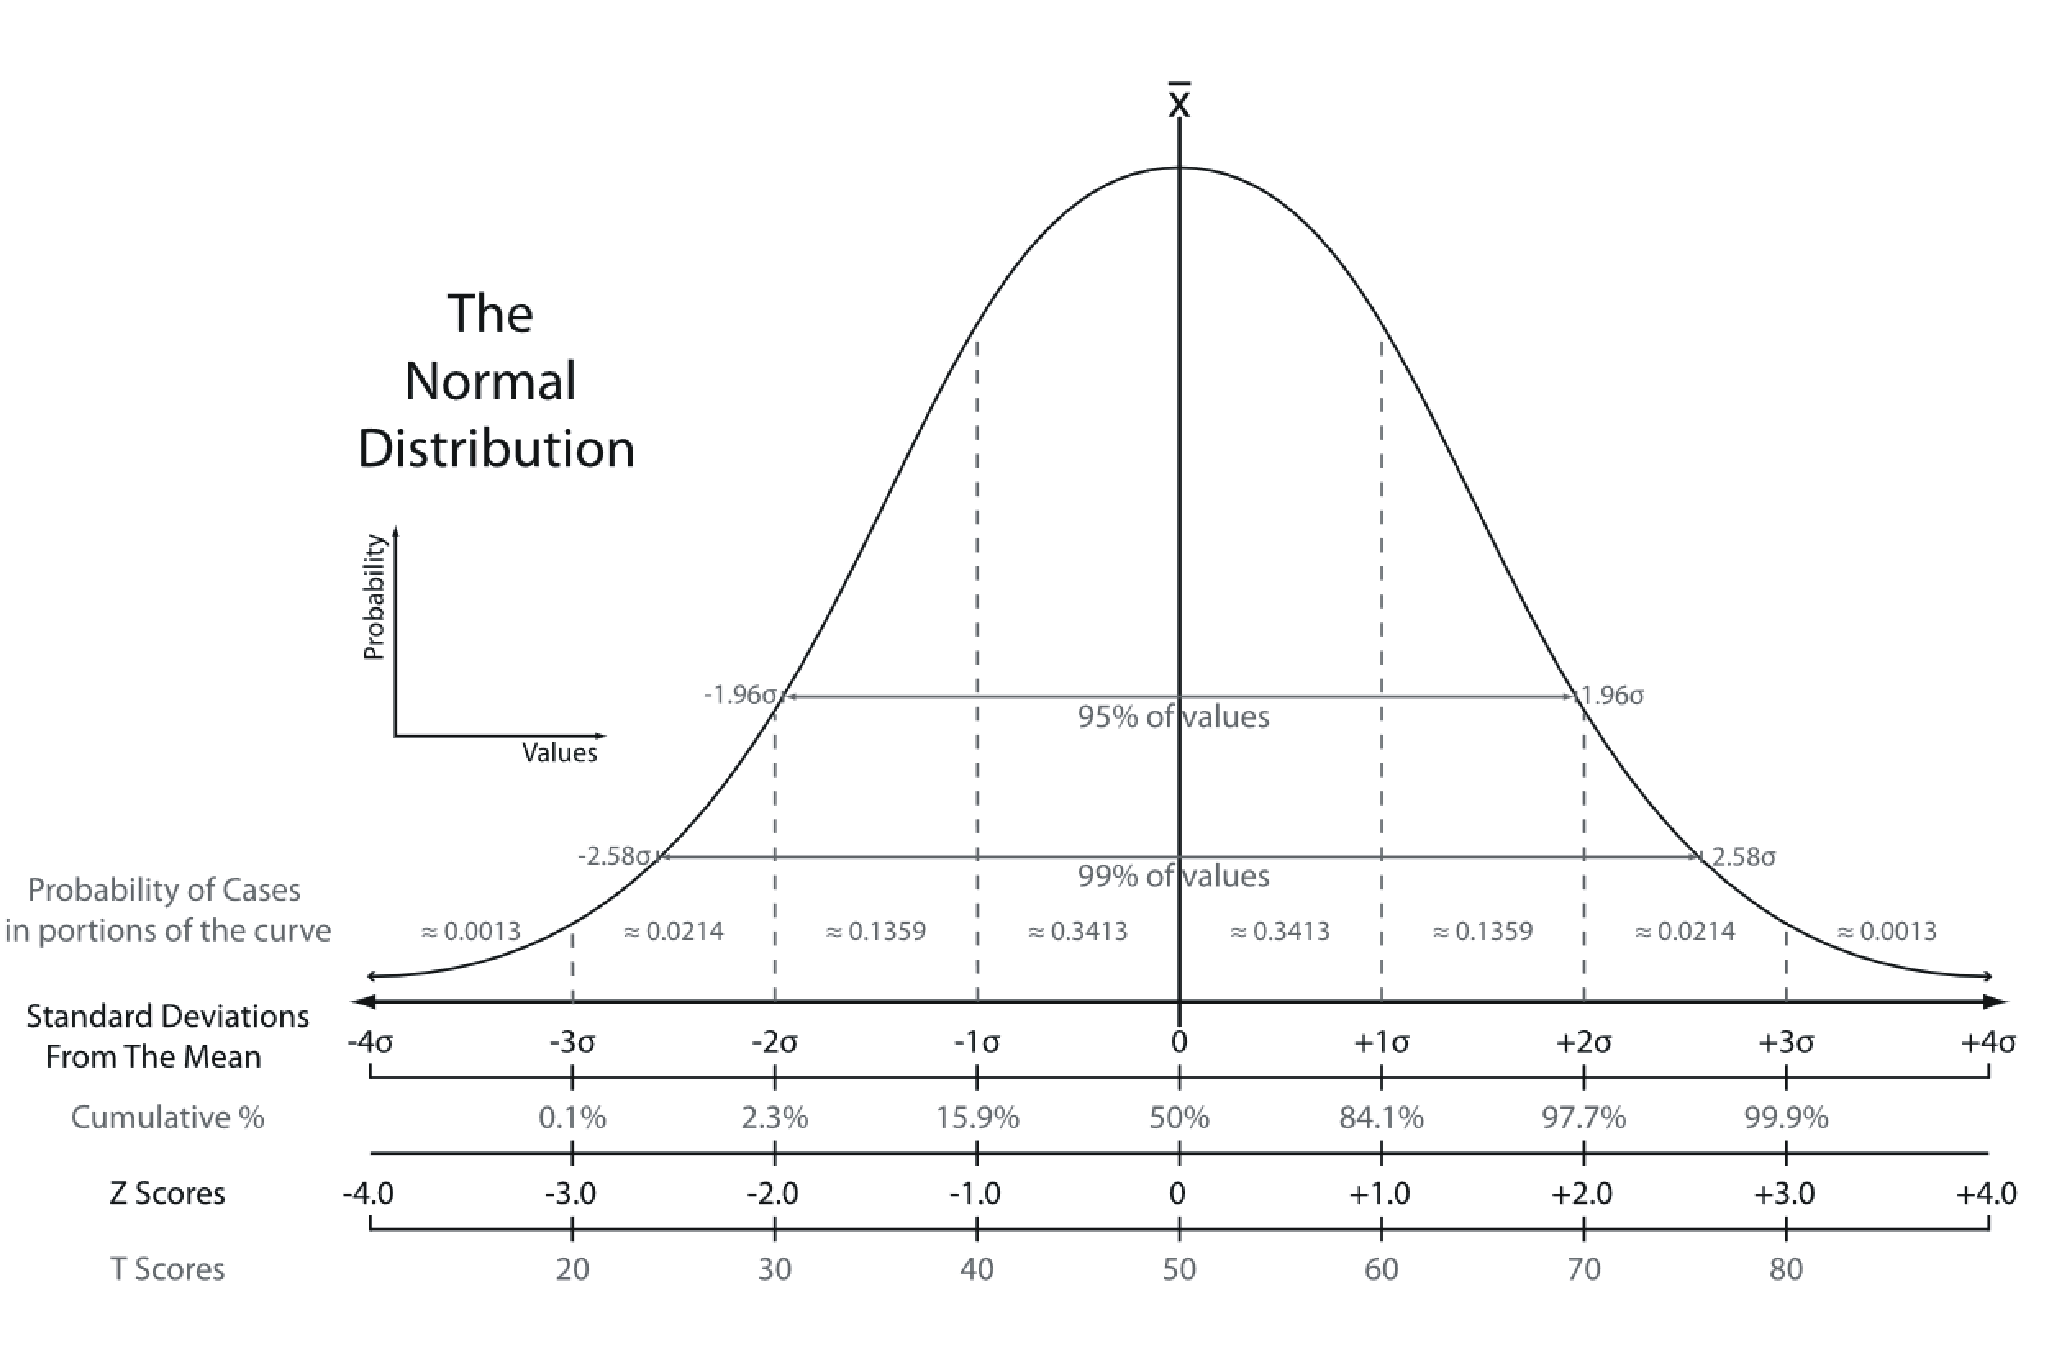
\includegraphics[width=150mm]{06_vorlesung/media/StandardScore.png}
		\caption{Die Standard-Normalverteilung $\mathcal{N}(0,\sigma^2)$ mit den entsprechenden Z-Werten.\newline 
		Quelle: https://en.wikipedia.org/wiki/Standard\_score }
		\label{fig:StandardScore}
	\end{center}
\end{figure}
In Abb.\ref*{fig:StandardScore} ist eine Standardnormalverteilung mit den 
Z-Scores (Z-Werten) dargestellt. 
Z-Scores können nur berechnet werden, wenn die zugrunde liegende Verteilung bekannt ist.
Im Falle von t-Tests haben wir hingegen auch die Möglichkeit auf die aus der Stichproben
geschätzten Parameter für den Erwartungswert und die Varianz zurückzugreifen.
In Abb.\ref*{fig:StandardScore} ist zusätzlich zu der Größe Z-Score ein  weitere
Größe aufgetragen: T-Score. Diese ist direkt proportional zu den Z-Scores nur mit einer
anderen Normierung, derart skaliert, dass ihr Erwartungswert $50$ ist und die
Standardabweichung den Wert $10$ annimmt. 

Entsprechend der internationalen Norm \cite{6_ISO13528} kann der Z-Wert für den Vergleich eines 
Messwertes $x_{i}$ eines Labors~$i$ mit dem Referenzwert $x_\mathrm{ref}$, der eine
Standardabweichung (Standardunsicherheit) $\sigma_\mathrm{ref}$ hat, verglichen werden.
Es wird folgender Z-Score berechnet und anschließend bewertet: 
\begin{equation}
 z_i = \frac{x_{i}-x_\mathrm{ref}}{\sigma_\mathrm{ref}}
\end{equation}
Nach \cite{6_ISO13528} gibt es die folgende übliche Interpretation für die Bewertung: 
\begin{itemize}
	\item Ein Ergebnis mit $|z_i| \le 2.0$ ist noch akzeptabel.
	\item Ein Ergebnis mit $ 2.0 < |z_i| < 3.0$ gibt ein Warnsignal.
	\item Ein Ergebnis mit $|z_i| \ge 3.0 $ wird als nicht akzeptierbar bewertet. 
\end{itemize}
Sind die erweiterten Unsicherheiten sowohl des Referenzlabors $U_\mathrm{ref}$ als auch 
des Teilnehmerlabors des $i$-ten Partners $U_{i}$ für das 
Überdeckungsintervall $[2 u; 2 u]$ zum 95,45\% Vertrauensniveau bekannt,
so kann der sogenannte \textbf{En-Wert} berechnet werden. 

In der vorigen Vorlesung hatten wir die Prüfgröße 
$T = \frac{x_1 - x_2}{\sqrt{s_1^2 + s_2^2}}$, die prüft ob zwei Stichproben mit ihren Erwartungswerten
$x_1$ und $x_2$ zur selben Grundgesamtheit gehören.
Dieser Hypothesentest prüft diese Größe auf $|T| > k$. Der Parameter $k$ steht hier allgemein für das Quantil,
also für $z_{1-\alpha/2}$ im Falle der Verwendung der Standardnormalverteilung wie sie hier in Abb.~\ref{fig:StandardScore}
dargestellt ist. Er steht für das Quantil $t_{1-\alpha/2,\nu}$ im Falle der Verwendung der t-Verteilung ($\alpha$: Signifikanzniveau, $\nu$:
Freiheitsgrad). Ferner steht der Parameter $k$ auch für das Quantil einer Posteriorverteilung, also den Faktor
eines \textsl{Credible} Intervalls, weshalb er allgemein \textsl{Erweiterungsfaktor} genannt wird.

Wenn wir eine Unsicherheit $u_i$ eines Labors vorliegen haben, die beispielsweise eine Standardabweichung $s_i$ sein kann, und haben wir ein symmetrisches Überdeckungsintervall, wie es bei normalverteilten oder t-verteilten Zufallsgrößen der Fall ist, so ist die halbe Breite des Überdeckungsintervalls $U_i = k u_i$. Dabei wird $U_i$ die \textsl{erweiterte Messunsicherheit} genannt.

Jetzt dividieren wir die Prüfgröße $T$ durch das Quantil bzw. den Erweiterungsfaktor $k$
$$
\frac{T}{k} = \frac{x_1 - x_2}{k \sqrt{s_1^2 + s_2^2}}  = \frac{x_1 - x_2}
{\sqrt{(k s_1)^2 + (k s_2)^2}} 
$$
und führen die bei Ringvergleichen allgemein verwendete Bezeichnung $E_n := T /k$ ein,
so dass die Prüfgröße mit $U_i = k u_i$ bzw.\  $U_i = k s_i$ wie folgt aussieht:
\begin{equation}
E_\mathrm{n} = \frac{x_{i}- x_\mathrm{ref}}{\sqrt{U_{i}^2+U_\mathrm{ref}^2}}
\label{eq:EnWert}
\end{equation}
Der \textbf{En-Wert} gibt an, wie gut der Laborwert $x_{i}$ mit dem 
Referenzwert $x_\mathrm{ref}$ übereinstimmt. Es werden hier die erweiterten Messunsicherheiten $U$ für $k=2$ kombiniert.
Da hier mit den erweiterten Unsicherheiten gerechnet wird, liegen die Grenzen der akzeptablen Werte nicht bei 2 sondern bei 1.
$|E_n|$ ist gemäß t-Test zu bewerten (siehe auch \cite{6_ISO13528}):
\begin{itemize}
	\item $|E_\mathrm{n}| < 1$: Die Nullhypothese wird angenommen und gilt als Indikator für eine gute Übereinstimmung
	\item $|E_\mathrm{n}| \ge 1$: Die Nullhypothese wird abgelehnt und gilt als Indikator, dass die Messdaten nicht konsistent zueinander sind.
\end{itemize} 

\section{Auswertung von Ringvergleichen ohne Referenzlabor}
\subsection{Vorgehensweise}
Ringvergleiche zwischen den NMIs (\textsl{National Metrology Institutes}), sog. 
\textbf{Key-Com\-pari\-sons} dienen u.a. dazu einen Referenzwert (KCRV: \textsl{key comparison reference
value}) mit einer zugeordneten Unsicherheit festzulegen.
Der Grad der Übereinstimmung der Messdaten von teilnehmenden Instituts $i$ zum Referenzwert ist hier gesucht. Es gibt keinen Referenzwert, weil man a priori nicht davon ausgehen kann, dass es ein Staatsinstitut gibt, das signifikant besser messen kann als alle anderen.
Ein mögliches Auswerteverfahren, das häufig Anwendung findet, ist bei 
\cite{6_Cox02} beschrieben. Bei diesem Auswerteverfahren müssen 
folgende 3 Voraussetzungen erfüllt sein: 
\begin{itemize}
	\item Jeder teilnehmende Partner $i$ ($i=1, \dots, N$) stellt Messdaten $x_i$ mit 
	beigeordneter Messunsicherheit $u(x_i)$ eines Prüflings bereit. Der 
	Prüfling muss eine gute Stabilität - auch während des Transportes -
	aufweisen. 
	\item Jeder Partner stellt Messdaten zur Verfügung, die 
	statistisch unabhängig von den anderen Partnern sind. D.h. es darf keine 
	Messung eines Partners $i$ von einem anderen Partner $j$ mit $i \ne j$ abhängen. 
	\item Die Messdaten jedes Partners (Instituts) sind normalverteilt.
\end{itemize}

Gegeben sind $N$ teilnehmende Institutionen mit $i=1,\dots,N$. Jeder
Partner/Institut $i$ stellt ein Messergebnis der Messgröße zur Verfügung, also einen Schätzwert $x_i$ und eine zugeordnete Standardmessunsicherheit
$u(x_i)$.
Der Ablauf der Auswertung sieht wie folgt aus:
\begin{itemize}
\item \textbf{Schritt 1:}  \newline
Da kein Referenzwert vorliegt, wird in diesem Fall ein gewichteter Mittelwert $\tilde x$ aus den Messergebnissen aller Partner bestimmt. Benutze dazu das inverse der Quadrate der zugeordneten Standardmessunsicherheiten als Gewichte: 
\begin{equation}
\tilde x = \frac{x_1/u^2(x_1)+ \cdots + x_N/u^2(x_N)}{1/u^2(x_1)+ \cdots 1/u^2(x_N)} = \frac{\sum\limits_{i=1}^{N} x_i / u^2(x_i)}
{\sum\limits_{i=1}^{N} u^{-2}(x_i)}
\label{eq:referenzgleichepartner}
\end{equation}
\item \textbf{Schritt 2:}  \newline
Bestimme die Standardabweichung des gewichteten Mittelwertes $u(\tilde x)=\sigma(\tilde x)$:
\begin{equation}
\frac{1}{u^2(\tilde x)} = \frac{1}{u^2(x_1)} +\cdots + \frac{1}{u^2(x_N)}
\label{eq:Standardabweichung_Mittelwert}
\end{equation}
\item \textbf{Schritt 3:}  \newline
Führe einen Konsistenzcheck durch, ob die angegeben Messergebnisse
konsistent zueinander sind. Führe dazu den $\chi^2$-Test
durch mit der $\chi^2$-Variablen (Testgröße $T$): 
\begin{equation}
T := \chi^2_\mathrm{obs} = \frac{(x_1 - \tilde x)^2}{u^2(x_1)} + \cdots + 
\frac{(x_n-\tilde x)^2}{u^2(x_N)}
\label{eq:T_for_consistencecheck}
\end{equation}
Diese Testgröße weist eher einen kleinen Wert auf, wenn alle Partner 
recht dicht am Mittelpartner liegen und natürlich umgekehrt. 
Vergleiche diese Testgröße mit der $\chi^2 (\nu)$ -Verteilung 
mit Freiheitsgrad $\nu = N-1$ ($N$ Anzahl der Partner), 
die am Messvergleich teilgenommen haben. 
Der Konsistenzcheck schlägt fehl, wenn die folgende Bedingung
erfüllt ist: 
\begin{equation}
\mathrm{Pr}\left(\chi^2(\nu) > T\right) < 0.05
\label{eq:consistencecheck}
\end{equation}
\glqq Pr\grqq~steht für \glqq Probability (Wahrscheinlichkeit)\grqq.
Der $\chi^2$-Test verlangt als Voraussetzung, dass die Messergebnisse
normalverteilt sind. 

\item \textbf{Schritt 4:}  \newline
Falls der Konsistenzcheck nicht fehlschlägt, wird der Wert $\tilde x$ als
Referenzwert (KCRV: key comparison reference value) $x_\mathrm{ref}$ akzeptiert
mit der Unsicherheit $u(x_\mathrm{ref}) = u(\tilde x)$. Nun kann der \textbf{Grad 
der Übereinstimmung} $d_i = x_i - x_\mathrm{ref}$ der Partner $i=1,\dots, N$ mit dem Referenzwert $x_\mathrm{ref}$ wie folgt bestimmt werden. 
Wir definieren die normierten Gewichte $\tilde w_i$
\begin{equation}
\tilde w_i := \frac{u^2(x_\mathrm{ref})}{u^2(x_i)}
\label{eq:anteile}
\end{equation}
mit
\begin{equation}
\sum_{i=1}^{N} \tilde w_i = 1 .
\label{eq:normierung}
\end{equation}
Der Referenzwert $x_\mathrm{ref} \equiv \tilde x$ aus Gl.~(\ref{eq:referenzgleichepartner}) ergibt sich wie folgt: 
\begin{equation}
x_\mathrm{ref} = \sum_{i=1}^{N} \tilde w_i\; x_i
\label{eq:referenzgleichepartner2}
\end{equation}

Für den Grad der Übereinstimmung erhalten wir: 
\begin{equation}
d_i = x_i - x_\mathrm{ref} = x_i - \sum_{j=1}^{N} \tilde w_j x_j 
= x_i - \tilde w_i x_i - \sum_{\substack{j=1 \\ j \neq i}}^{N} \tilde w_j x_j 
= (1-\tilde w_i)x_i - \sum_{\substack{j=1 \\ j \neq i}}^{N} \tilde w_j x_j 
\end{equation}
Wenn die Messungen nicht gegenseitig voneinander abhängen, so kann 
zur Berechnung der Unsicherheit von $d_i$ das Gesetz der Fortpflanzung
der Unsicherheiten angewendet werden. (Hinweis: Sind ein Modell mit $y=f(x_1, x_2)$ und 
die dazugehören Unsicherheiten $u(x_1)$ sowie $u_(x_2)$ gegeben, so ergibt sich die Unsicherheit von
$y$ bei Nichtkorrelation von $x_1$ und $x_2$ nach dem Gesetz der Fehlerfortpflanzung zu: 
$u^2(y)=\left(\frac{\partial f}{\partial x_1}\right)u^2(x_1)+\left(\frac{\partial f}{\partial x_2}\right)u^2(x_2)$)

Für die Unsicherheit der Differenz $d_i$ ergibt sich somit:
\begin{eqnarray}
u^2(d_i) &=& \left( \frac{\partial d_i}{\partial x_i} \right)^2 \cdot u^2(x_i) +  \sum_{\substack{j=1 \\ j \neq i}}^{N}
\left( \frac{\partial d_i}{\partial x_j} \right)^2 \cdot u^2(x_j) \\
&=&  (1-\tilde w_i)^2 u^2(x_i) + \sum_{\substack{j=1 \\ j \neq i}}^{N} \tilde w_j^2 u^2( x_j) \\
&=& ((1-\tilde w_i^2)-\tilde w_i^2)u^2(x_i) + \sum_{j=1}^{N} \tilde w_j^2 u^2(x_j) 
\end{eqnarray}
Mit Gl.(\ref{eq:anteile}) ergibt sich:
\begin{equation}
u^2(d_i) = (1-2\tilde w_i^2)u^2(x_i) + \sum_{j=1}^{N} \tilde w_j u^2(x_\mathrm{ref}) 
\end{equation}
Mit Gl.(\ref{eq:anteile}) und Gl.(\ref{eq:normierung}) ergibt sich daraus:
\begin{eqnarray}
u^2(d_i) &=& u^2(x_i) - 2u^2(x_\mathrm{ref}) + u^2(x_\mathrm{ref}) \sum_{j=1}^{N}\tilde w_j  
\nonumber \\
  &=& u^2(x_i) -u^2(x_\mathrm{ref})
\end{eqnarray}
Auch hier kann nun wieder ein En-Wert angeben werden. Da alle Größen normalverteilt sind, sind die erweiterten Unsicherheiten für einen 
Erweiterungsfaktor von $k=2$, $U(x_i) = k \cdot u(x_i) =2 \cdot u(x_i)$. Damit lässt sich der En-Wert mit Gl.(\ref{eq:EnWert}) bestimmen, der den
Grad der Übereinstimmung des beteiligten Partners $i$ mit dem Referenzwert
angibt.
\begin{equation}
E_\mathrm{n}(x_i) = \frac{d_i}{2\sqrt{u^2(d_i)}}
\end{equation}
\end{itemize}

Es gelten wieder die Aussagen von Kapitel 1:
\begin{itemize}
	\item $|E_\mathrm{n}| < 1$ ist ein Indikator für eine gute Übereinstimmung.
	\item $|E_\mathrm{n}| \ge 1 $ ist ein Indikator, dass die Messdaten nicht konsistent zueinander sind.
\end{itemize} 
\subsection{Beispiel}
\label{Beispielringvergleich1}
% \textbf{Beispiel} \newline
5 Partner messen ein Massestück von ca. 100 g. Die Ergebnisse 
der Partner sind wie folgt (alle Angaben sind in g):
\begin{center}
\begin{tabular}{l | c c c c c}
$i$	& 1 & 2 & 3 & 4 & 5 \\	\hline
$x_i / \mathrm{g}$ & 99.82 &  99.05 & 99.17 & 99.20 & 99.38  \\ \hline
$u(x_i) / \mathrm{g}$ & 0.80 & 0.63 & 0.86 & 0.82 & 0.98  
\end{tabular}
\end{center}
Als Ergebnis erhalten wir: $x_\mathrm{ref} = 99.29$ und $u_\mathrm{ref} = 0.35$. 
Mit der Testgröße $T=0.6239$ ergibt sich die Wahrscheinlichkeit 
$\mathrm{Pr}\{\chi^2(\nu) > T\} = 0.8858$. Da die Wahrscheinlichkeit größer als 0.05 ist, schlägt der
Konsistenzcheck nicht fehl, 
d.h.\ die Daten der 5 Messpartner sind konsistent.

Für die Abweichungen $d_i$ erhalten wir: 
$$
[0.7172 \;\;   0.5209 \;\;   0.7836  \;\;  0.7395 \;\;   0.9137]. 
$$
Für die En-Werte erhalten wir: 
$$
[ 0.3676 \;\;  -0.2329 \;\;  -0.0783 \;\;  -0.0626 \;\;   0.0478].
$$
Das heisst der Partner 5 ist in bester Übereinstimmung mit dem Referenzwert. \\
Der Octave-/Matlab-Code dazu lautet (Hinweis zu Octave: Evtl. ist die Funktion
\texttt{chi2pdf} in Octave noch nicht vorhanden. Dann zuerst das Paket statistics
installieren, \texttt{pkg install -forge package\_name} mit 
\texttt{package\_name = statistics} und evtl. den Pfad hinzufügen): \\
% z.~B. \texttt{addpath('C:\textbackslash Octave\textbackslash
% Octave-4.2.1\textbackslash share\textbackslash octave\textbackslash packages')}
\begin{lstlisting}[style=Matlab]
% addpath('C:\Octave\Octave-4.2.1\share\octave\packages');
% clear all;
x = [99.82, 99.05, 99.17 , 99.20 ,99.38];
u_x = [0.80 0.63, 0.86, 0.82, 0.98];
U_x = 2*u_x;

% Anzahl der Freiheitsgrade
nu = 4;

% Schritt 1:
x_ref = sum(x./(u_x).^2) ./ sum(1./(u_x).^2)

% Schritt 2: 
u_ref = sqrt(1./sum(1./(u_x).^2))

% Schritt 3: 
T = sum((x-x_ref).^2./(u_x.^2))

% Bestimme die Wahrscheinlichkeit Pr der Chi^2-Verteilung fuer Chi^2(\nu) > T:
Pr = 1 - chi2pdf(T,nu)

% Schritt 4: Grad der Uebereinstimmung
d = x-x_ref;
u_d = sqrt(u_x.^2 - u_ref.^2)
En = d./(2*sqrt(u_d.^2))
\end{lstlisting}

\subsection{Identifikation von Ausreißern und Konsistenzcheck}
Wir wollen uns hier noch etwas genauer anschauen, wie man feststellt, 
ob die Messdaten eines Ringvergleiches konsistent sind und wie man mit Inkonsistenten umgeht.
Als \textbf{Ausreißer} werden häufig Messwerte deklariert, deren Abweichungen größer  
als 3 mal die erweiterte Messunsicherheit des Referenzwertes \cite{6_GuideKey} sind.
Diese Ausreißer werden in Abstimmung mit dem Partner gelöscht. 
Anschließend werden die verbliebenen Daten auf statistische Konsistenz
überprüft. Wir haben dazu bereits in Gl.(\ref{eq:T_for_consistencecheck}) und Gl.(\ref{eq:consistencecheck}) 
eine Formel angegeben, mit der überprüft werden kann, ob die angegebenen
Messergebnisse (Messwerte mit Unsicherheiten) konsistent zu dem Referenzwert und 
dessen Unsicherheit ist. Die Testgröße $T$ basiert auf dem Birge-Test, 
welche ebenso ein Test auf die Konsistenz der Messdaten in einem Ringvergleich
ist. Der Birge-Test ist wie der $\chi^2$-Test nur unter folgenden Bedingungen
gültig:
\begin{itemize}
	\item Die gemessenen Messwerte $x_i$ der $N$ Institute sind unkorreliert
	\item Man benötigt Kenntnis über die Verteilungsdichtefunktionen. Es 
	wird vorausgesetzt, dass die Größen normalverteilt mit den Unsicherheiten $u(x_i)$ bzw. den Varianzen $\sigma_i$ sind.
\end{itemize}
Das Birge-Verhältnis ist -bis auf die Anzahl der Freiheitsgrade- die Prüfgröße des Chi2-Tests (siehe vorherige Vorlesung) 
% Gl.~\ref{chi2testgroesse}).
Es wird folgendes geprüft ($H_0$: Nullhypothese, $H_a$: Alternativhypothese):
\begin{center}
	\begin{tabular}{l | p{14cm} }
	$H_0$	& $u_\mathrm{partner}^2 =  u_\mathrm{ref}^2$:\newline 
	Die Stichprobe gehört zu 
		einer Grundgesamtheit  mit Varianz $u_\mathrm{ref}^2$\\	\hline
 $H_\mathrm{a}$	& $u_\mathrm{partner}^2 \neq  u_\mathrm{ref}^2$: \newline 
 Die Stichprobe gehört nicht zu einer Grundgesamtheit mit Varianz $u_\mathrm{ref}^2$\\ 
	\end{tabular}
\end{center}
 
Das \textbf{Birge-Verhältnis} ist definiert als das Verhältnis der Streuungen der Unsicherheiten aller Partner 
(bezeichnen wir mit $u_\mathrm{partner}$) zu der Unsicherheit des Referenzwertes $u_\mathrm{ref}$. Es wird
analog der Testgröße des $\chi^2$-Tests, $T = \nu \left(\frac{s}{\sigma_0}\right)^2$ Gl.~\ref{chi2testgroesse}, wie
folgt definiert:
\begin{equation}
R_\mathrm{B} := \frac{u_\mathrm{partner}}{u_\mathrm{ref}}
\quad \text{mit} \quad 
\frac{u^2_\mathrm{partner}}{u^2_\mathrm{ref}} \, \propto \, 
\nu \left(\frac{s}{\sigma_0}\right)^2.
\end{equation}
Die Varianz aller $N$ Partner ist wie folgt definiert:
\begin{equation}
u^2_\mathrm{partner} := \frac{\frac{1}{N-1} \sum\limits_{i=1}^{N} w_i \left(x_i-x_\mathrm{ref} \right)^2}
{\sum\limits_{i=1}^{N} w_i} \quad \text{mit} \quad w_i = \frac{1}{u^2(x_i)} .
\end{equation}
Entsprechend Gl.(\ref{eq:Standardabweichung_Mittelwert}) ist die Unsicherheit des Referenzwertes wie folgt gegeben
\begin{equation}
u_\mathrm{ref} = \left(\frac{1}{u^2(x_1)} +  \cdots + \frac{1}{u^2(x_N)} \right)^{-\frac{1}{2}},
\end{equation}
so dass für das Birge-Verhältnis gilt
\begin{equation}
R_\mathrm{B} = \sqrt{\frac{1}{N-1} \; \sum_{i=1}^N \left( \frac{x_i-x_\mathrm{ref}}{u(x_i)} \right)^2 }.
		\label{eq:Birge-Verhaeltnis}
\end{equation}

Vergleicht man das Birge-Verhältnis mit der Testgröße $T = \nu \left(\frac{s}{\sigma_0}\right)^2$ in Gl.(\ref{eq:T_for_consistencecheck}) so ergibt sich der Zusammenhang:
\begin{equation} 
R_\mathrm{B}^2 = \frac{1}{N-1} \; T
\end{equation}
Bei dem Konsistenzcheck mit dem Birge-Verhältnis wird untersucht, ob  
\begin{itemize}
	\item $R_\mathrm{B} \le 1$: Konsistenzcheck ok. 
	\item $R_\mathrm{B} > 1$: Konsistenzcheck schlägt fehl.
\end{itemize}
Wenn $R_\mathrm{B} > 1$ ist, bedeutet dies, dass entsprechend Gl.(\ref{eq:Birge-Verhaeltnis}) die Unsicherheiten der Partner 
$u(x_i)$ nicht zu der Unsicherheit des Referenzwertes $u(x_\mathrm{ref})$ passen.
Die gemessenen Daten $x_i$ der Partner sind inkonsistent.
Für unser Beispiel Abschnitt \ref{Beispielringvergleich1} erhalten wir $R_\mathrm{B} = 0.39494$.
Damit schlägt der Birge-Test nicht fehl und die Daten sind 
danach konsistent. Für die Auswertung eines Ringvergleichs ist es empfehlenswert sowohl das Birge-Verhältnis als auch den $\chi^2$-Test
(siehe Gl.(\ref{eq:consistencecheck})) durchzuführen und zu prüfen, ob beide Tests ok sind. 

Häufig wird das Birge-Verhältnis in Gl.(\ref{eq:Birge-Verhaeltnis}) 
umgeschrieben und in folgender Form dargestellt:
\begin{equation}
R_\mathrm{B}^2 = \sum_{i=1}^N \frac{w_i (x_i - x_\mathrm{ref})^2}{N-1}
\end{equation}
mit den Gewichten $w_i = 1/\sigma_i^2$ für $i=1,2,\ldots, N$ und dem 
Referenzwert (gewichteten Mittelwert) $x_{ref}=\sum_i w_i x_i / \sum_i w_i$.
Der Birge Test kann auch bei korrelierten Messdaten $x_1,\ldots ,x_N$, wenn die 
Kovarianzen $\sigma_{12},\ldots, \sigma_{(N-1)N}$ gegeben sind, durchgeführt werden, siehe \cite{6_Kac08}.

\subsection{Paule-Mandel Methode zur Anpassung von Gewichtsfaktoren}

Bei Ringvergleichen kommt es auch mal vor, dass die Messmethoden nicht immer genau die gleichen sind und der Einfluss der verschiedenen Methoden des Vergleichs unterschätzt wird. Wenn sich herausstellt, dass sich Gruppen von Ergebnissen ausbilden, so kann eine Zwischengruppenvarianz ermittelt werden. Dies kann beispielsweise mit der Paule-Mandel Methode erfolgen.

Es kann bei Ringvergleichen vorkommen, dass jeder am Vergleich beteiligte Partner eine
Unsicherheit $U$ angibt, die kleiner ist als der Abstand des Messwertes zu anderen Partnern,
so dass sich ein En-Wert bzw.\ des Birge-Verhältnisses unter Verwendung der Gewichte gemäß Gl.~(\ref{eq:anteile}) größer als Eins ergibt. Durch eine Anpassung der Gewichtsfaktoren durch Hinzufügen einer
zusätzlichen Komponente, die sich aus der Streuung der Ergebnisse von Partner zu Partner ergibt, kann eine bessere Konsistenz erzielt werden.

Der Leitfaden zum Erstellen eines \textsl{Key Comparison Reports}
\cite{GuideKey} empfiehlt als Anpassungsverfahren die \textbf{Paule-Mandel Methode},
bei der die Varianzen durch Additions einer Streuung zwischen Laboratorien
erhöht werden. Dadurch werden die Gewichtsfaktoren $w_i$ verkleinert und damit Referenzwert 
$x_\mathrm{ref}$ so angepasst, so dass das Birge-Verhältnis kleiner als Eins werden kann.
Ein Beispiel dazu ist im Anhang B der Richtlinie für Ringvergleiche \cite{GuideKey} zu finden.

Im Folgenden schauen wir uns das Prinzip von Mandel und Paule an, das 
in der Publikation \cite{Pau82} zu finden. Es werden zwei eher künstliche Beispiele gewählt, um das Prinzip besser zu verstehen. 
In Beispiel I wird eine Messgröße mit zwei verschiedenen Methoden (bzw.\ von zwei verschiedenen Partnern) A und B gemessen.
Die gemessenen Einzelwerte von jedem der beiden Partner sind in Tab. \ref*{tab:Beispiel_I}
angegeben.
\begin{table}[!htb]
	\caption{Messdaten des Beispiels I}
	\begin{center}
	\begin{tabular}{l| rrr |rrr}
		\hline 
		Methode/Partner & \multicolumn{3}{c}{A} \vline & \multicolumn{3}{c}{B} \\ \hline
		Gemessener Wert $x_i$ & 1.1 & 1.9 & 1.5 & 16 & 25 & 3 \\ \hline
	\end{tabular}
\end{center}
\label{tab:Beispiel_I}
\end{table}

Der gleichgewichtete Mittelwert $\bar x_I$ über alle Werte beider Partner ist:
 \begin{equation}
 \bar x_I = \frac{1}{N} \sum_{i=1}^N x_i \, = \frac{1}{6}\left( 1.1 + 1.9 + 1.5 + 16 + 25 + 3 \right) \, \approx \, 8.1
 \end{equation}
 Intuitiv würden wir jedoch sagen, dass wir den Messdaten mit der Methode A
 mehr vertrauen schenken würden, als den Messdaten mit der Methode B, da die 
 Messdaten der Methode A weniger streuen als die Messdaten mit der Methode B.

 Als zweites Beispiel betrachten wir, dass die Methoden (bzw. Partner) A und B ähnlich
 genau messen, jedoch werden von Partner A einen größeren Stichprobenumfang
 als von Partner B:

 
 \begin{table}[!htb]
 	\caption{Messdaten des Beispiels II}
 	\begin{center}
 		\begin{tabular}{l| rrrrrr |rr}
 			\hline 
 			Methode/Partner & \multicolumn{6}{c}{A} \vline & \multicolumn{2}{c}{B} \\ \hline
 			Gemessener Wert $x_i$ & 2.0 & 1.0 & 1.5 & 1.8 & 1.2 & 1.7 
 			& 16.3 & 16.8\\ \hline
 		\end{tabular}
 	\end{center}
 	\label{tab:Beispiel_II}
 \end{table}
Für den gleichgewichteten Mittelwert über alle Werte erhalten wir:
 \begin{equation}
 \bar x_{II} = \frac{1}{N} \sum_{i=1}^N x_i \, = \frac{1}{8}\left( 2.0 + 1.0 + 1.5 + 1.8 + 1.2 + 1.7 + 16.3 + 16.8 \right) \, = \, 5.2875
\label{eq:einfachesMittelII}
 \end{equation}
Es fällt auf, dass die beiden Werte von Partner B zueinander passen, sich aber deutlich von denen von Partner A unterscheiden.

Die beiden Mittelwerte der jeweiligen Partner A und B sind
 \begin{equation}
 \bar x_{II,A} = \frac{1}{6}\left( 2.0 + 1.0 + 1.5 + 1.8 + 1.2 + 1.7 \right) = 1.533, 
\quad \bar x_{II,B} = \frac{1}{2}\left( 16.3 + 16.8 \right) = 16.550
 \label{eq:Mittelwerte_x_II_A_B}
 \end{equation}

\begin{comment}

\textcolor{red}{\textbf{Dieses würde ich hier an dieser Stelle gar nicht bringen, auch wenn es in Pau82 
so präsentiert wird, weil Du ja hier in diesem Skript schon mit den Gewichten als Kehrwert
der Varianzen für den Referenzwert, der aus dem gewichteten Mittel der Resultate aller Partner
gewonnen wurde, um En-Werte für gleiche Partner zu bestimmen.}}


\textcolor{red}{zunächst hatte ich entlang am Pau82 die Sachen so nachgerechnet und verstanden, wie
Paule und Mandel sie argumentiert hatte, dann wurde mir langsam klar, dass wir in unseren Vorlesungen
aber längst an dem Punkt angekommen sind, dass man die Kehrwerte der Varianzen nimmt und nicht
anfängt die Mittelwerte einfach zu mitteln $\Rightarrow$ alles Blaue hiernach hier wegnehmen}

\textcolor{blue}{und der Mittelwert dieser beiden Mittelwerte ist
 \begin{equation}
  \bar x_{II,AB} = \frac{1}{2}\left( 1.533 + 16.550 \right) = 9.0417
 \label{eq:Mittelwerte_x_IIAB}
 \end{equation}
 Dadurch dass wir Mittelwerte mitteln erhalten wir eine andere Wichtung: $\frac{\sum w_i x_i}{\sum w_i}$:
$$
\frac{1}{2} \left( \frac{1}{6} \left(\sum\limits_{i=1}^6 x_i \right) \; + \;
    \frac{1}{2} \left(\sum\limits_{i=7}^8 x_i \right)  \right) =
 \frac{1}{12} \left(\sum\limits_{i=1}^6 x_i \right) \; + \;
    \frac{1}{4} \left(\sum\limits_{i=7}^8 x_i \right)
$$
also 
$$
\frac{w_i}{\sum\limits_{i=1}^8 w_i} \, = \, 
\left\{ \begin{array}{ccl}
\frac{1}{12} & \text{f{\"u}r} & i = 1,\dots,6 \\
\frac{1}{4} & \text{f{\"u}r} & i = 7, 8
\end{array} \right.
$$
Diese Art der Wichtung, die Einzelwerte zu gewichten, führt dazu dass Stichprobe B
sehr viel stärker gewichtet wird, in diesem Beispiel um einen Faktor $3$ mit $\frac{1}{4} = \frac{3}{12}$.
Es macht jedoch mehr Sinn, die Gewichte danach zu richten, wie genau die Größen sind,
im Sinne von der Frage wie breit oder schmal die Wahrscheinlichkeitsdichteverteilung ist.}
\end{comment}

Wir haben im Laufe dieser Vorlesungsreihe bereits gesehen, dass
Messergebnisse mit größerer Unsicherheit sinnvollerweise mit geringerer
Wichtung zu berücksichtigen sind, so dass Gewichte
deshalb aus dem Kehrwert der Varianzen bestimmt werden. Der Grund dafür liegt darin,
dass die Varianz des gewichteten Mittelwertes $x_\mathrm{ref}$ minimiert wird,
wenn die Gewichte als Reziprokwert der Varianzen der Einzelwerte berechnet werden.
In Gl.~(\ref{eq:referenzgleichepartner2}) 
haben wir deshalb zur Ermittlung des Referenzwertes $x_\mathrm{ref}$ beim
Ringvergleich mit gleichwertigen Partnern gerechnet mit
\begin{equation*}
    w_i = \frac{1}{u^2_i}
\end{equation*}
und
\begin{equation*}
 x_\mathrm{ref} = \frac{\sum\limits_{i=1}^N w_i x_i}{\sum\limits_{i=1}^N w_i} .
\end{equation*}

\begin{comment}
\textcolor{red}{wahrscheinlich macht es keinen Sinn mit der empirischen Varianz
anzufangen, sondern direkt mit der empirischen Var des Mittelwertes, also nehme ich
diesen Teil wieder zurück}
\textcolor{blue}{Verwenden wir für die Unsicherheit $u_i$ die empirische Varianz
$u_i = \operatorname{Var}(x_i)$ für Beispiel II folgende Werte
$$
\operatorname{Var}(x_{II,A}) = 
\frac{1}{6-1} \sum\limits_{k=1}^{6} \left(x_{II,k} - \bar x_{II,A} \right)^2 = 0.14267
$$
und
$$
\operatorname{Var}(x_{II,B}) = \frac{1}{2-1} \sum\limits_{k=7}^{8} \left(x_{II,k} - \bar x_{II,B} \right)^2
= 0.12500
$$ 
so erhalten wir für die beiden Gewichte $w_A = 7.0093$ und $w_B = 8.0000$, die beide fast gleich.
Der gewichtete Mittelwert, der als Referenzwert für En-Tests und das Birge-Verhältnis genutzt wird ist damit
$$
x_\mathrm{ref} \; = \; \frac{7.0093 \cdot 1.533 \; + \; 8.0000 \cdot 16.550}{7.0093 + 8.0000}
\; = \; 9.5372
$$
Nach Gl.~(\ref{eq:Birge-Verhaeltnis}) das Birge-Verhältnis hierfür
$$
R^2_\mathrm{B} \; = \; \frac{1}{N-1} \; \sum_{i=1}^N \left( \frac{x_i-x_\mathrm{ref}}{u^2(x_i)} \right)^2 \; = \;
 \frac{1}{2-1} \, \left( \frac{\left(1.5333 - 9.5372\right)^2}{0.14267}
 \, + \, \frac{ \left( 16.550 - 9.5372 \right)^2}{0.12500} \right) = 842.47 \gg 1
$$
--nix!}
\end{comment}

Wenn die Varianzen 
der Methode A und B ähnlich sind, so kann eine gemeinsame (gepoolte) Varianz der beiden Methoden berechnet werden (siehe 5. Vorlesung):
\begin{equation}
\operatorname{Var}(x_{ref}) = \frac{\sum\limits_{i=1}^6 \left(x_{A,i}-\bar x_A\right )^2+\sum\limits_{i=1}^2 \left(x_{B,i}-\bar x_B\right )^2}{(6-1)+(2-1)} = 0.1397
\end{equation} 

Da es sich um den Vergleich der Mittelwerte der beiden Stichproben A und B handelt, verwenden wir
für die Unsicherheit $u_i$ die Varianz des Mittelwertes, also
$u_i = \operatorname{Var}(\bar x_i)$. Sie ist definiert als
$$
\operatorname{Var}(\bar x_i) = \frac{\operatorname{Var}(x_i)}{N_i}
$$
mit $N_i$ den Anzahl der Wiederholungen für den Mittelwert $\bar x_i$.

Für Beispiel II erhalten wir dann folgende Werte:
$$
\operatorname{Var}(\bar x_{II,A}) = \frac{1}{6(6-1)} \sum\limits_{k=1}^{6} \left(x_{II,k} - \bar x_{II,A} \right)^2 = 0.023778
\quad \text{d.h.} \quad \bar s_A = \sqrt{\operatorname{Var}(\bar x_{II,A})} = 0.154
$$
und
$$
\operatorname{Var}(\bar x_{II,B}) = \frac{1}{2(2-1)} \sum\limits_{k=7}^{8} \left(x_{II,k} - \bar x_{II,B} \right)^2 = 0.062500
\quad \text{d.h.} \quad \bar s_B = \sqrt{\operatorname{Var}(\bar x_{II,B})} = 0.250
$$
so erhalten wir für die beiden Gewichte $w_A = 42.056$ und $w_B = 16.000$.
Der gewichtete Mittelwert, der als Referenzwert für En-Tests und das Birge-Verhältnis genutzt wird, ist damit
$$
x_\mathrm{ref} \; = \; \frac{42.056 \cdot 1.533 \; + \; 16.000 \cdot 16.550}{42.056 + 16.000}
\; = \; 5.6716
$$
Nach Gl.~(\ref{eq:Birge-Verhaeltnis}) das Birge-Verhältnis hierfür
$$
R^2_\mathrm{B} \; = \; \frac{1}{N-1} \; \sum_{i=1}^N \left( \frac{x_i-x_\mathrm{ref}}{u(x_i)} \right)^2 \; = \;
 \frac{1}{2-1} \, \left( \frac{\left(1.5333 - 5.6716\right)^2}{0.023778}
 \, + \, \frac{ \left( 16.550 - 5.6716 \right)^2}{0.0625} \right) = 2613.7
$$
also
$$
R_\mathrm{B} \; = \; \sqrt{2613.7} \, = \, 51.1  \gg 1
$$

% https://iopscience.iop.org/article/10.1088/0026-1394/51/5/516/meta

Wir sehen, dass die Varianzen der Mittelwerte der beiden Partner A und B im Verhältnis zur
Differenz zwischen den beiden Partnern sehr klein ist, oder umgekehrt gesagt liegen die 
Mittelwerte der Methoden A und B sehr weit auseinander im Verhältnis zu den Varianzen.
Die Varianzen $\operatorname{Var}(\bar x_A)$ und $\operatorname{Var}(\bar x_A)$ beschreiben
nur die interne Streuung, also nur die Streuung der jeweiligen Stichproben A und B.
Die Wahrscheinlichkeitsverteilungen werden durch die beiden Parameter Erwartungswert,
also hier Mittelwert und Varianz charakterisiert und wir hatten bei den Hypothesentests
gelernt, auf beides zu prüfen. Wir haben gesehen, dass Stichproben einer gemeinsamen
Grundgesamtheit angehören, wenn beides, Mittelwert und Varianz zueinander passen.

Bei den Ringvergleichen, bei denen von verschiedenen Laboratorien oder Instituten mit
unterschiedlichen Methoden oder jedenfalls unabhängigen experimentellen Aufbauten die
Ergebnisse verglichen werden, kann beobachtet werden, dass entweder die
Schätzer (empirischen Erwartungswerte) oder die empirischen Varianzen oder sogar
beides nicht zusammen passen. In der Praxis kommt es vor, dass die jeweiligen
Labore oder Institute ihre Methode immer weiter optimiert haben und ihre Genauigkeit
erhöht haben, dass jedoch verbleibende, unerkannte systematische Effekte vorhanden sind.
Dass es Unterschiede gibt, tritt erst bei dem Vergleich zutage und es lässt sich
im Rahmen der gesetzten Zeit für das Projekt des Vergleichens nicht aufklären.
In solchen Fällen lebt man dann damit, dass es auch zwischen den unterschiedlichen
Methoden bzw.\ Laboren eine Streuung gibt.

Statistisch wird dies damit ausgedrückt, dass die Stichproben auf den verschiedenen
Laboren zu verschiedenen Grundgesamtheiten gehören.
Konkret bedeutet das, dass für die Gewichte zusätzlich zur Varianz des Mittelwert
zur jeweiligen Methode/ des jeweiligen Laboratoriums
(Streuung innerhalb einer Gruppe, \textsl{within group variability})
auch eine Varianz der Methoden/Laboratorien (Streuung zwischen Gruppen,
\textsl{between group variability}) eingeführt.
Die Streuung zwischen den Gruppen, die Varianz $s^2_\mathrm{b}$ wird
iterativ geschätzt. Für die verschiedenen Partner oder Stichproben $A$ und $B$
verwenden wir jetzt die Notation $S_i$, hier also $S_1 = A$ und $S_2 = B$, um
die Gleichungen allgemein aufschreiben zu können.
\begin{equation*}
\operatorname{Var}(\bar x_{S_i,\mathrm{c}}) \; = \;
\operatorname{Var}(\bar x_{S_i}) \; + \; s^2_\mathrm{b} \; = \;
\frac{1}{M_i (M_i - 1)} \sum\limits_{k \in S_i}
\left( x_{k} - \bar x_{S_i} \right)^2 
\; + \; s^2_\mathrm{b}
\end{equation*}
mit $M_i$ für den Stichprobenumfang zu $S_i$ -
oder kürzer aufgeschrieben mit $i$ als Index für die Nummerierung der Partner
und für die Varianzen der Mittelwerte bzw.\ Messergebnisse 
der Partner
$u^2_i = \bar s^2_i = \operatorname{Var}(\bar x_{S_i})$
bzw.\ für die Konsensusvarianzen
$\bar s^2_{i,\mathrm{c}} = \operatorname{Var}(\bar x_{S_i,\mathrm{c}})$
\begin{equation}
\bar s^2_{i,\mathrm{c}} \; = \; \bar s^2_j \; + \; s^2_\mathrm{b}
\label{eq:consensusVariability}
\end{equation}
wobei der Index b für \textsl{between} und c für \textsl{consensus}
stehen. Auch die Mittelwerte bzw.\ allgemein die Messergebnisse der
jeweiligen Partner schreiben wir jetzt in der Form $\bar x_{S_i} = \bar x_i$.

Die Gewichte für den \textsl{Consensus Value}, dem besser übereinstimmenden
Wert für die Messgröße, sind damit dann
\begin{equation*}
w_{i,\mathrm{c}} \, = \; \frac{1}{\operatorname{Var}(\bar x_{S_i,\mathrm{c}})} \; = \;
\left(\frac{1}{M_i (M_i - 1)} \sum\limits_{k \in S_i}
\left( x_{k} - \bar x_{S_i} \right)^2 
\; + \; s^2_\mathrm{b} \right)^{-1}
\end{equation*}
mit $M_i$ für den Stichprobenumfang zu $S_i$ 
und dasselbe in der kürzeren Notation geschrieben
\begin{equation}
w_{i,\mathrm{c}} \, = \, \frac{1}{\bar s^2_{i,\mathrm{c}}} \, = \, \frac{1}{\bar s^2_j \; + \; s^2_\mathrm{b}} .
\label{eq:consensusWeights}
\end{equation}
Der Konsenzreferenzwert aus den Werten aller $N$ Partner ist dann
\begin{equation}
x_\mathrm{ref, c} \, = \, 
\frac{\sum\limits_{i=1}^N w_{i,\mathrm{c}} x_i}{\sum\limits_{i=1}^N w_{i,\mathrm{c}} }.
\label{eq:consensusMean}
\end{equation}
Das Birge-Verhältnis für diese Konsensuswerte ist somit
\begin{equation}
R_\mathrm{B} \; = \; \sqrt{ \frac{1}{N-1} \, \sum\limits_{i=1}^N
\frac{1}{\bar s^2_i \; + \; s^2_\mathrm{b}} \, \left(\bar x_i - x_\mathrm{ref, c}\right)^2}.
\end{equation}

\textbf{Schätzen der Zwischengruppenvarianz $s^2_\mathrm{b}$}
\begin{quote}
Geschätzt wird die Zwischengruppenvarianz $s^2_\mathrm{b}$ gemäß Paule und Mandel \cite{Pau82} als
diejenige Varianz, für die die Ergebnisse der Partner konsistent sein sollen, also für die
das Birge-Verhältnis gegen Eins streben soll: $R_\mathrm{B} \rightarrow 1$.
\end{quote}
Die Optimierungsaufgabe formulieren wir für das Quadrat des Birge-Verhältnisses,
um eine Kostenfunktion zu haben, die sich einfacher linearisieren lässt. Dies
geht ganz gut, weil $1^2 = 1$ ist, also $R^2_\mathrm{B} \rightarrow 1$, d.h.
\begin{equation*}
\frac{1}{N-1} \, \sum\limits_{i=1}^N
\frac{1}{\bar s^2_i \; + \; s^2_\mathrm{b}} \, \left(\bar x_i - x_\mathrm{ref, c}\right)^2 \rightarrow 1
\end{equation*}
oder genauer ausgedrückt
\begin{equation}
\min_{s^2_\mathrm{b}} \left\{\frac{1}{N-1} \, \left( \sum\limits_{i=1}^N
\frac{1}{\bar s^2_i \; + \; s^2_\mathrm{b}} \, \left(\bar x_i - x_\mathrm{ref, c}\right)^2  \right) \, - \, 1\right\}.
\label{eq:x_bet_Bedingung}
\end{equation}

Diese Optimierungsaufgabe hat eine Kostenfunktion 
$Q(s^2_\mathrm{b}) = \frac{1}{N-1} \, \left( \sum\limits_{i=1}^N 
\frac{1}{\bar s^2_i \; + \; s^2_\mathrm{b}} \, \left(\bar x_i - x_\mathrm{ref, c}\right)^2  \right) \, - \, 1$
die von dem zu schätzenden Parameter, der Zwischengruppenvarianz
$v := s^2_\mathrm{b}$ nicht-linear abhängt, so dass sie iterativ zu lösen ist, es handelt sich also
nichtlineare Optimierung wie wir es in Kapitel~\ref{nonlinOpti} besprochen haben.

Wir entwickeln die Kostenfunktion in 
eine Taylorreihe bis zum linearen Term
\begin{equation}
Q(v_0 + \operatorname{d} v_0) \approx 
Q_0 + \left.\left( \frac{\partial Q}{\partial v}\right)
\right|_{v=v_0} \operatorname{d} v_0 
\end{equation}
Mit $Q(v) \rightarrow 0$ setzen wir für den ersten
Iterationsschritt
\begin{equation}
Q_0 + \left.\left( \frac{\partial Q}{\partial v}\right)
\right|_{v=v_0} \operatorname{d} v_0 = 0
\end{equation}
und lösen dies nach $\operatorname{d} v_0$ auf zu
\begin{equation}
\operatorname{d} v_0 = -\left. \left( \frac{Q_0}{\frac{\partial Q}{\partial v}}\right) \right| _{v=v_0} 
\end{equation}
Wir beginnen mit dem Startwert für $v_0$, indem wir ihn auf $v_0 = 0$ setzten, so dass wir
mit dem sehr großen Birge-Verhältnis beginnen und iterativ die Zwischengruppenvarianz
erhöhen, um das Birge-Verhältnis solange zu reduzieren bis es Eins wird.
Im nächsten Schritt setzen wir $v_1 = v_0 + \operatorname{d} v_0$.
Dies setzten wir fort mit
\begin{equation}
v_{k+1} =v_k + \operatorname{d} v_k
\end{equation}
bis $Q$ zu einem Minimum möglichst nahe bei Null konvergiert.

Die Ableitung der Kostenfunktion $Q$ nach der Zwischengruppenvarianz ist
\begin{equation*}
\frac{\partial Q}{\partial v} = \frac{1}{N-1} \, \left( \sum\limits_{i=1}^N 
\frac{\partial }{\partial v} \frac{1}{\bar s^2_i \; + \; v} \, \left(\bar x_i - x_\mathrm{ref, c}\right)^2  \right) \, - \, 0
\end{equation*}
d.h.
\begin{equation*}
\frac{\partial Q}{\partial v} = \frac{1}{N-1} \, \sum\limits_{j=1}^N  \left(\bar x_j - x_\mathrm{ref, c}\right)^2 
\frac{\partial }{\partial v} \frac{1}{\bar s^2_i \; + \; v} 
\end{equation*}
d.h.
\begin{equation}
\frac{\partial Q}{\partial v} = \frac{1}{N-1} \, \sum\limits_{i=1}^N  \left(\bar x_i - x_\mathrm{ref, c}\right)^2 
\frac{-1}{\left(\bar s^2_i \; + \; v\right)^2} 
\end{equation}
Die Iterationen laufen, solange $R_\mathrm{B}$ größer als Eins ist und eine maximale Anzahl Iterationsschritte einen Wert von $50$ nicht überschreitet.
In dem hier behandelten Beispiel werden $17$ Iterationsschritte gebraucht, bis die
Optimierung konvergiert und folgendes Ergebnis für die Zwischengruppenvarianz $v = s^2_\mathrm{b}$ liefert.

$$
v = 112.707 \quad \text{d.h.} \quad s_\mathrm{b} = 10.6
$$

\begin{comment}
\textcolor{red}{ich werde hier noch einen Plot erzeugen, der die Gaußverteilungen der
beiden Einzelstichproben zeigt (vielleicht außerdem noch die t-Verteilungen) sowie die
Gaußverteilung ${\cal N}(x_\mathrm{ref} = 9.040, s_\mathrm{b} = 10.6)$ für die
Zwischengruppenverteilung.}
\end{comment}
Die Konsensusvarianz für den Referenzwert können wir dann wie folgt berechnen: 
$$
\operatorname{Var}(x_\mathrm{ref}) = \left(\sum\limits_{i=1}^N \frac{1}{\bar s^2_i \; + \; s^2_\mathrm{b}}\right)^{-1}
= 56.375;  \quad s_\mathrm{ref} = \sqrt{\operatorname{Var}(x_\mathrm{ref})} = 7.5
$$
Als Ergebnis ergibt sich damit:
\begin{equation}
x_\mathrm{ref} = 9.040 \quad \text{mit} \quad
s_\mathrm{ref} = 7.5
\end{equation}

\begin{figure}[!htp]
	\begin{center}
		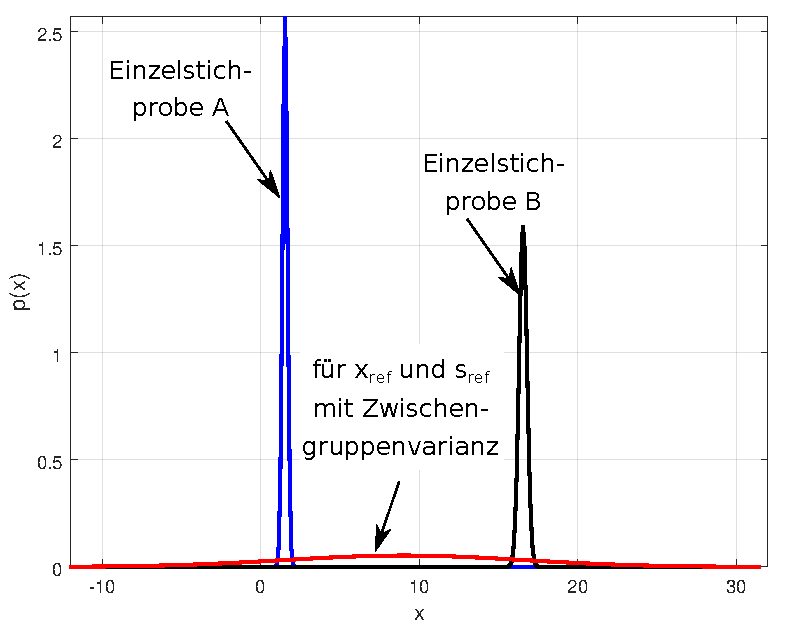
\includegraphics[width=120mm]{06_vorlesung/media/PauleMandel.pdf}
		\caption{Wahrscheinlichkeitsdichteverteilungen als Normalverteilungen
  zu Beispiel II mit blauer Kurve für die Einzelstichprobe A mit $\bar x_{II,A} = 1.533$
  und $\bar s_A = 0.1542$, schwarzer Kurve für die Einzelstichprobe B mit $\bar x_{II,B} = 16.550$
  und $\bar s_B = 0.2500$, sowie die gemeinsame Verteilung nach Hinzufügen der Zwischengruppenvarianz mit
  $x_\mathrm{ref} = 9.040$ und $\sqrt{\operatorname{Var}(x_\mathrm{ref})} = 7.5$ als sehr viel breitere und
  flachere Gaußverteilung dargestellt als rote Kurve.}
		\label{fig:Pau82BeispielII}
	\end{center}
\end{figure}

Der dazu gehörige Quellcode für Gnu-Octave/Matlab sieht wie folgt aus: 
\begin{lstlisting}[style=Matlab]
function consensus_fit()
% Programm laeuft unter Matlab und Gnu-Octave
x_A = [2.0,1.0,1.5,1.8,1.2,1.7];
N_A = length(x_A);
x_B = [16.3,16.8];
N_B = length(x_B);

bar_x_A = mean(x_A);
bar_x_B = mean(x_B);
fprintf('Mittelwerte: %f und %f \n', bar_x_A, bar_x_B);

% Varianzen der Mittelwerte
Var_A_mittel = var(x_A)/N_A;
Var_B_mittel = var(x_B)/N_B;
fprintf('Varianzen der Mittelwerte innerhalb jeder Stichprobe: \n %f und %f \n'...
,  Var_A_mittel, Var_B_mittel);

% Anzahl der Methoden/ Partner M
M = 2;
% Startwert fuer Zwischengruppenvarianz
v_0 = 0;

% Berechnung des Birge ratio fuer den Startwert
w_A = 1/Var_A_mittel;
w_B = 1/Var_B_mittel;
x_ref = (w_A*bar_x_A + w_B*bar_x_B ) / (w_A + w_B);
RB = sqrt( (1/(M-1))*(w_A * (bar_x_A - x_ref)^2 + ...
w_B * (bar_x_B - x_ref)^2));
fprintf('Birge-Verhaeltnis fuer den Startwert %f\n\n',RB)
% 
max_num_iterations = 50;
v = v_0;
k = 0;
while (RB > 1) && (k < max_num_iterations)
w_A = 1/(Var_A_mittel + v);
w_B = 1/(Var_B_mittel + v);

x_ref = (w_A*bar_x_A + w_B*bar_x_B ) / (w_A + w_B);
RBsq = (1/(M-1))*(w_A * (bar_x_A - x_ref)^2 + ...
w_B * (bar_x_B - x_ref)^2);
RB = sqrt(RBsq);
Q = RBsq - 1;
dQ_dv = (-1/(M-1))*(w_A^2 * (bar_x_A - x_ref)^2 + ...
w_B^2 * (bar_x_B - x_ref)^2);
dv = -Q / dQ_dv;
v = v + dv;
k = k + 1;
fprintf('x_ref: %f, RB: %.3f, dv: %e --> v: %.3f\n', x_ref, sqrt(RBsq), dv,v);
end
fprintf('\n s_b = %f bei Anzahl Iterationen %d\n', ...
sqrt(v-dv), k);
end
\end{lstlisting}
mit dem Output:
\begin{lstlisting}[style=Matlab]
>> consensus_fit
Mittelwerte: 1.533333 und 16.550000 
Varianzen der Mittelwerte innerhalb jeder Stichprobe: 
0.023778 und 0.062500 
Birge-Verhaeltnis fuer den Startwert 51.123910

x_ref: 5.671861, RB: 51.124, dv: 4.312238e-02 --> v: 0.043
x_ref: 7.356441, RB: 36.154, dv: 8.619528e-02 --> v: 0.129
x_ref: 8.198732, RB: 25.569, dv: 1.721928e-01 --> v: 0.302
x_ref: 8.619877, RB: 18.087, dv: 3.435958e-01 --> v: 0.645
x_ref: 8.830449, RB: 12.799, dv: 6.840440e-01 --> v: 1.329
x_ref: 8.935734, RB: 9.064, dv: 1.355587e+00 --> v: 2.685
x_ref: 8.988376, RB: 6.429, dv: 2.661878e+00 --> v: 5.347
x_ref: 9.014695, RB: 4.574, dv: 5.132109e+00 --> v: 10.479
x_ref: 9.027851, RB: 3.273, dv: 9.539961e+00 --> v: 20.019
x_ref: 9.034421, RB: 2.371, dv: 1.649219e+01 --> v: 36.511
x_ref: 9.037690, RB: 1.756, dv: 2.470307e+01 --> v: 61.214
x_ref: 9.039294, RB: 1.357, dv: 2.797615e+01 --> v: 89.190
x_ref: 9.040038, RB: 1.124, dv: 1.861186e+01 --> v: 107.802
x_ref: 9.040319, RB: 1.022, dv: 4.691663e+00 --> v: 112.494
x_ref: 9.040375, RB: 1.001, dv: 2.129841e-01 --> v: 112.707
x_ref: 9.040377, RB: 1.000, dv: 4.038510e-04 --> v: 112.707
x_ref: 9.040377, RB: 1.000, dv: 1.446530e-09 --> v: 112.707
x_ref: 9.040377, RB: 1.000, dv: 0.000000e+00 --> v: 112.707

s_b = 10.616355 bei Anzahl Iterationen 18
\end{lstlisting}
\nopagebreak 
\begin{thebibliography}{-----------}
	\item[] \hspace*{5em}{\Large\bf zu Kapitel 6:}
	\bibitem[Cox02]{6_Cox02} M. G. Cox: The evaluation of key comparison data, Metrologia 39, 589-595 (2002)
	\bibitem[ISO13528]{6_ISO13528} ISO: Statistical methods for use in proficency testing by interlaboratory comparison, Second edition 2015-08-01, corrected version 2016-10-15
	\bibitem[Kac08]{6_Kac08} R.N.Kacker, A.B.Forgbers
	R. N. Kacker, A. B. Forbes, R. Kessel and K. Sommer Bayesian posterior predictive
	p-value of statistical consistency in interlaboratory evaluations Metrologia 45 512-523 (2008)
	\bibitem[GuideKey]{6_GuideKey} Guidelines for CCPR Key Comparison Report
	Preparation, https://www.bipm.org/utils/common/pdf/CC/CCPR/CCPR-G2.pdf
	\bibitem[Pau82]{6_Pau82}  R.C. Paule, J. Mandel: Consensus Values and Weighting Factors, J. Res. NBS, Vol.87, No.5,377-385 (1982)
\end{thebibliography}
